% Vertx Instalation process
%
% External sources
%

\newpage
\section*{Instalación de Gradle}
	\paragraph{Para sistemas basados en Unix (Linux y Mac).}
	\paragraph{Para poder tener los módulos de Ambienta2MX corriendo es necesario contar con una versión de la máquina virtual de java en ejecución, o bien un JDK (Java Development Kit), curl, git o wget (véase la instalación de dichas bibliotecas en el sistema de su preferencia), a continuación se muestra :}
	\begin{alltt}
		curl -s http://get.sdkman.io | bash
	\end{alltt}
	\paragraph{Para poder instalar las versiones necesarias de Groovy, Vertx y Gradle se utilizarán los siguientes comandos.}
	\begin{alltt}
		sdk install gradle
	\end{alltt}:
	\paragraph{Después de instalar gradle, se puede acceder a la carpeta de los fuentes, ``HardAnt'', ``FastEagle'' o ``SmartOwl'' y ejecutar el siguiente comando:}
	\paragraph{Mostrando finalmente el acceso al gestor como lo muestra la siguiente imagen.}
	\begin{alltt}
		gradle tasks
	\end{alltt}:
	\paragraph{Esto bajará las bibliotecas a usar por el proyecto y mostrará todas las tareas que dependen de éste, como se muestra en la siguiente captura de pantalla.}
  \paragraph{Ahora es necesario realizar la creación de la base de tipo Places (Fast Eagle), utilizando la siguiente línea en una terminal nueva.}
  \begin{figure}[h!]
	\centering
		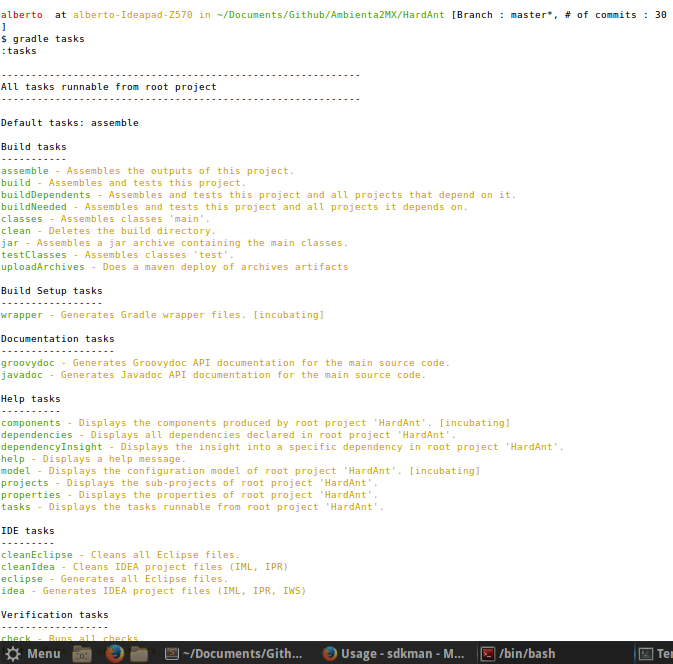
\includegraphics[width=\textwidth]{./images/TerminalGradle}
		\caption{Tareas de Gradle en el proyecto Hard Ant.}
  \end{figure}  
\addcontentsline{toc}{chapter}{Anexo 5: Instalación de Gradle} 